\section{Overall Framework}
\begin{figure*}
    \centering
    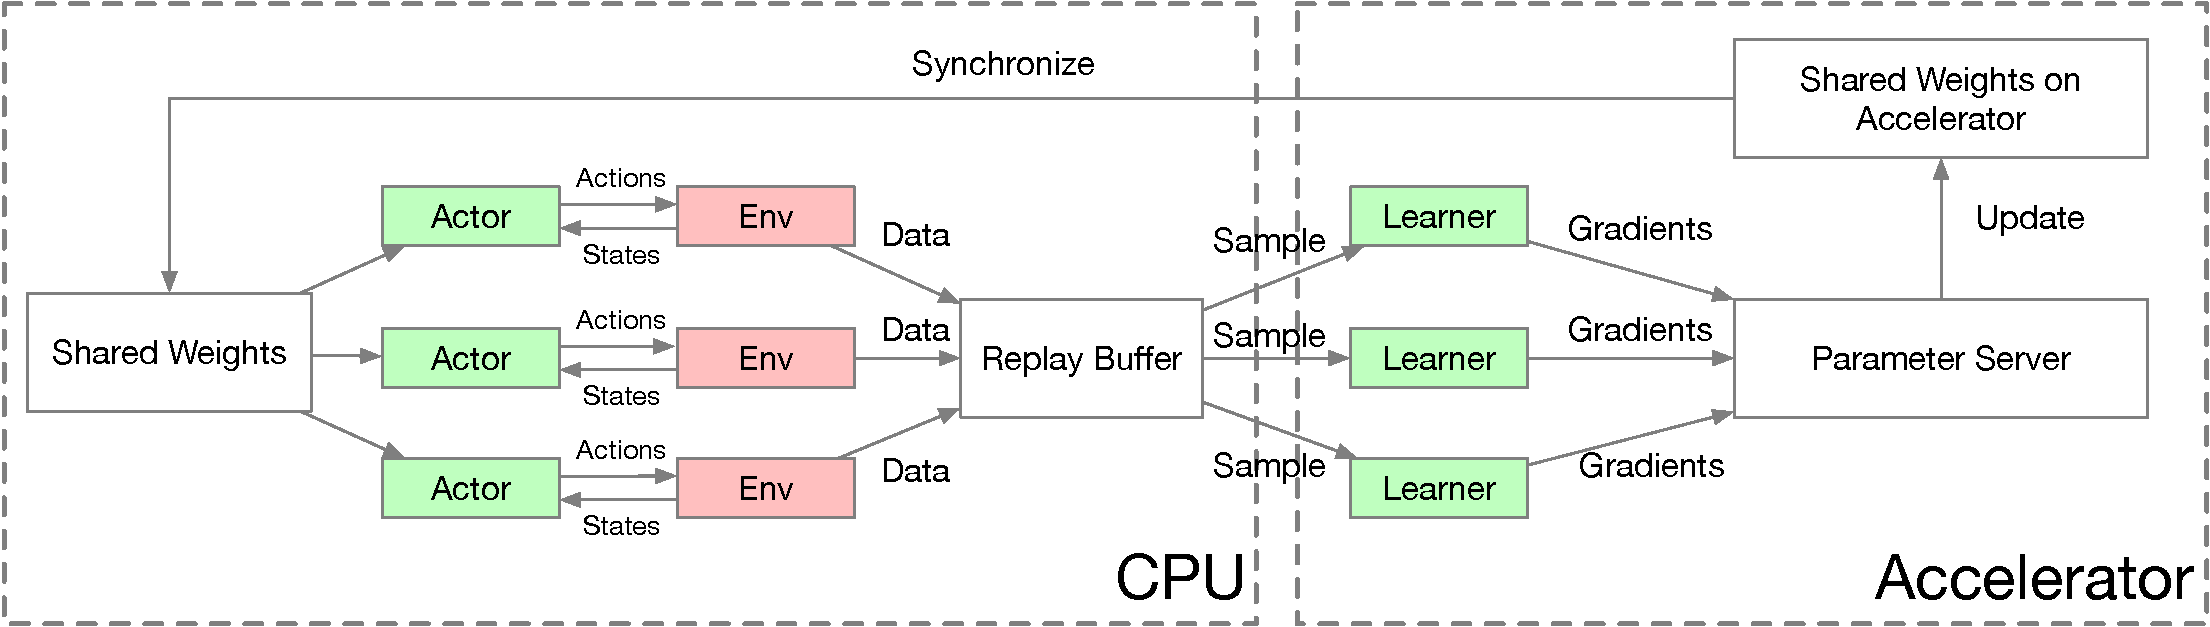
\includegraphics[width=\linewidth]{overall_system.pdf}
    \caption{Overall system architecture}
    \label{fig:overall_system}
\end{figure*}

The overall system architecture is shown in Figure~\ref{fig:overall_system}. We employ parallel actors to collect data and parallel learners to compute the gradients for neural network weights update. 

\subsection{Asynchronous Actors}
Asynchronous actors collect the data simultaneously by interacting with their own instance of the environment using the shared weights. The data is then added to the Replay Buffer. It is worth noting that no synchronization is required because the inference doesn't alter the weights.

\subsection{Parallel Learners}
Deploying parallel actors increases the throughput of data collection. In order to increase the throughput of the learning, we employ parallel learners with a central parameter server \cite{parameter_server}. Each learner independently samples one batch of data from the Replay Buffer and computes the sub-gradients. The parameter server aggregates the gradients and updates the weights.

\subsection{Framework Specification}
Our framework supports a wide range of reinforcement learning algorithms including DQN \cite{dqn}, DDQN \cite{double_q_learning}, DDPG \cite{ddpg}, SAC \cite{sac}, TD3 \cite{td3} and so on. The target platform of our framework is processor + accelerator platforms, where the processor is the CPU the accelerator is either the GPU or the FPGA. The input of our framework includes:
\begin{itemize}
    \item The overall throughput of the data collection vs. the number of CPU cores.
    \item The overall throughput of the data consumption vs. the number of CPU cores.
    \item Total number of cores in the CPU.
\end{itemize}
The throughput of the data collection by a single actor is affected by i) the time of a single environment step function defined in Section~\ref{sec:mdp}; ii) The specifications of the neural networks used in the actors including the architecture (fully-connected vs. convolution networks), the size of each layer, etc. iii) the speed of the processor. The throughput of a single learner is affected by i) the reinforcement learning algorithm; ii) the optimizer iii) the speed of the accelerator.

\subsection{Design Space Exploration}\label{sec:design_space_exp}
The objective of is to choose the number of actor threads and the number of learner threads such that the ratio between the throughput of the data collection vs. data consumption is the same as the single thread implementation (update\_interval denoted in Algorithm~\ref{alg:off_policy_rl}). In order to obtain the allocation of the cores, we profile the overall throughput of the data collection vs. the number of CPU cores and denote the curve as $f_{a}(x)$, where $x$ is the number of cores. Similarly, we profile the overall throughput of the data consumption vs. the number of CPU cores and denote the curve as $f_{l}(x)$. Let the total number of CPU cores be $M$. Then, the design space exploration is the solution of equation~\ref{eq:design_space}:
\begin{align}
    \label{eq:design_space}
    f_{a}(x_a) &= \text{update\_interval}\times f_{l}(x_l) \nonumber\\
    x_a + x_l &\leq M
\end{align}
where $x_a$ and $x_l$ is the allocated number of cores for actors and learners, respectively.
If the parallel actors and/or learners are deployed on an accelerator such as GPU or FPGA, instead of CPU, profiling similar to the one described above can be used to perform the design space exploration. 
